%#! platex main.tex

%======================================================================
\chapter{提案手法}

本章では, 食事中に発生する音から食事内容を推定し, 咀嚼を検出する手法について述べる.

\begin{figure}[t]
    \centering
    \begin{tabular}{c}
        \begin{minipage}{0.6\hsize}
            \centering
            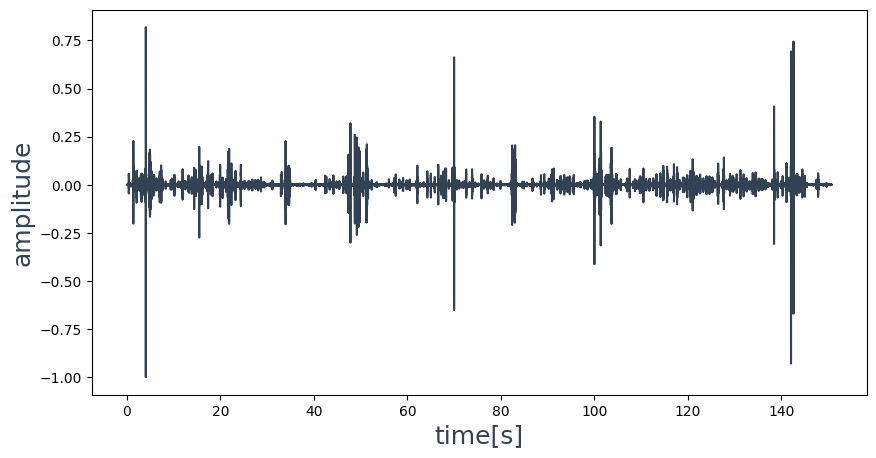
\includegraphics[width=1.0\hsize]{img/sound-example-rice.png}
            \subcaption{ご飯}
            \label{fig:sample-data-rice}
        \end{minipage}
        \\
        \\
        \begin{minipage}{0.6\hsize}
            \centering
            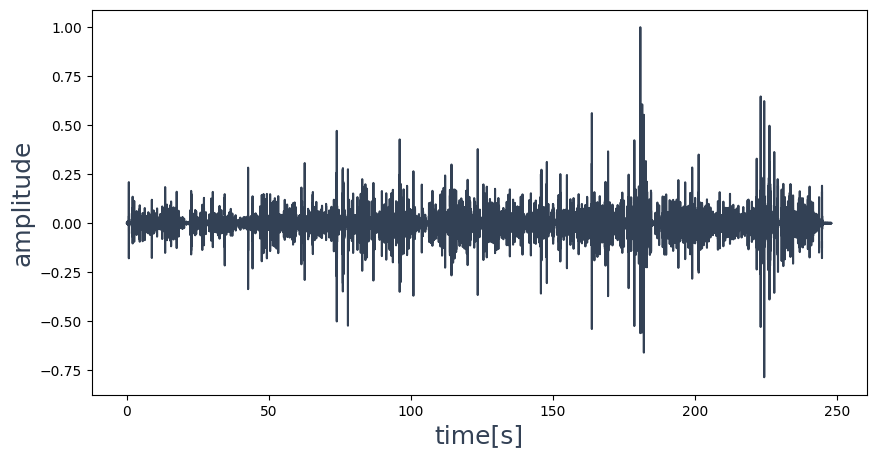
\includegraphics[width=1.0\hsize]{img/sound-example-salad.png}
            \subcaption{サラダ}
            \label{fig:sample-data-salad}
        \end{minipage}
        \\
        \\
        \begin{minipage}{0.6\hsize}
            \centering
            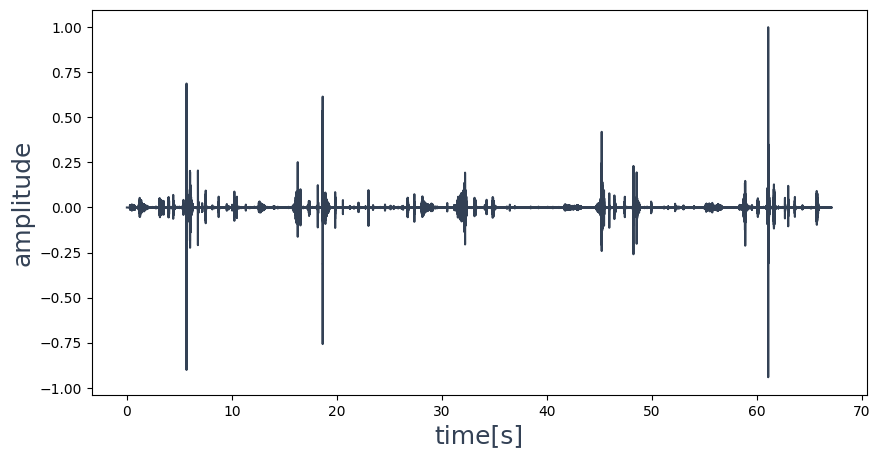
\includegraphics[width=1.0\hsize]{img/sound-example-soup.png}
            \subcaption{味噌汁}
            \label{fig:sample-data-soup}
        \end{minipage}
    \end{tabular}
    \caption{録音データの波形の一例}
    \label{fig:sample-data}
\end{figure}

\begin{figure}[t]
    \begin{center}
        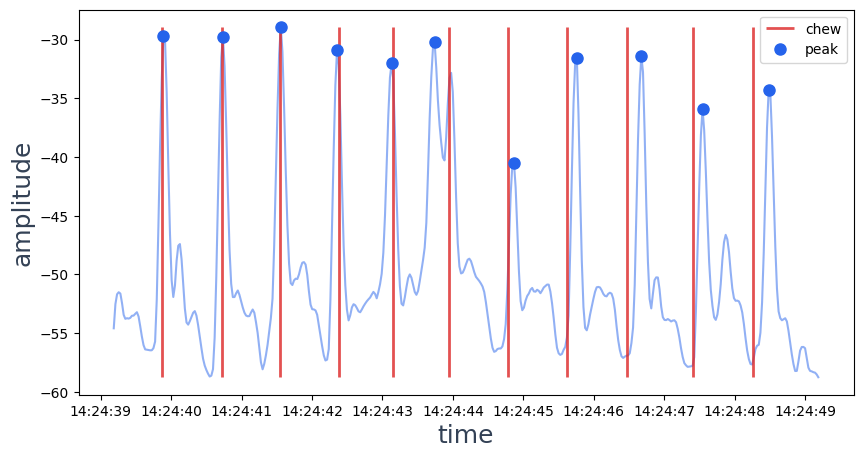
\includegraphics[clip,  width=0.95\hsize]{img/peak-sample.png}
        \caption{ピーク検出}
        \label{fig:peak-sample}
    \end{center}
\end{figure}

\begin{figure}[t]
    \begin{center}
        \includegraphics[clip,  width=0.95\hsize]{img/food.png}
        \caption{対象とする食品}
        \label{fig:foods}
    \end{center}
\end{figure}

%----------------------------------------------------------------------
\section{食事内容の推定}

本稿では, 食事中の録音データをメルスペクトログラムに変換し, 畳み込みニューラルネットワークによる学習を行うことで, 食事内容推定モデルを生成する. メルスペクトログラムを用いてCNNで音声分類を行うと従来の手法よりも精度が出ることが言われているため\cite{Dossou_2021_ICCV}, 本研究でもこの手法を採用する.
食事中に発生する音をウィンドウ幅$500ms$, オーバーラップ率$0.75$のスライディングウィンドウで部分時系列データに分割する. ただし, 最大信号強度が$-65dBFS$以下のデータと音の長さが$500ms$に満たないものは除外する. 特徴抽出のために, スライディングウィンドウでセグメントされた音データに対して, メルスペクトログラムを算出する. これらのデータを訓練データ$90\%$とテストデータ$10\%$に分割し, 訓練データを用いて畳み込みニューラルネットワークCNNを学習させる. CNNには4つの畳み込み層を使用し, 畳み込み層の後に一つの最大値プーリング層とドロップアウト層を使用する. 最後の層はソフトマックス層である. 最終的に, テストデータを用いて学習済みモデルの精度評価を行う.

%----------------------------------------------------------------------
\section{咀嚼の検出}

音声信号処理においてオンセット検出は一般的な手法であり, スペクトルエネルギ分布からピークを検出することで, 音楽イベントを自動で検出することができる. 本稿でも, 咀嚼イベントの検出にオンセット検出を採用する. 食事中の音をメルスペクトログラムに変換し, 各時間軸毎の全ての周波数帯の信号強度の平均を取り, ピークを検出することで, 咀嚼の検出を行う. 図\ref{fig:peak-sample}にピーク検出の例を示す. 評価については, 10秒間の音データに対して被験者がカウントした咀嚼回数とピーク検出回数との間の平均絶対値誤差$MAE$を算出する. $MAE$の算出式は以下に示す.

\begin{equation}
    \text{MAE} = \frac{1}{n} \sum_{i=1}^{n} | y_i - \hat{y}_i |
\end{equation}

\begin{table}[t]
    \centering
    \caption{被験者データ}
    \label{personaldata}
    \scalebox{0.85}{
        \begin{tabular}{c|c|c|c}
            \hline
            \textbf{被験者} & \textbf{年齢} & \textbf{性別} & \textbf{計測した食品}                                                                   \\ \hline\hline
            A            & 22          & 男           & \begin{tabular}{c}唐揚げ,クリームパン,グラタン\\ハンバーグ,ご飯,せんべい\\サラダ,味噌汁,焼きそば,ヨーグルト\end{tabular} \\ \hline
            B            & 23          & 男           & クッキー,ポテトチップス                                                                      \\ \hline
            C            & 22          & 男           & \begin{tabular}{c}クッキー,焼き魚,ハンバーグ\\スパゲティ,ヨーグルト\end{tabular}                        \\ \hline
            D            & 23          & 男           & クッキー,クリームパン,せんべい                                                                  \\ \hline
            E            & 23          & 男           & ご飯,サラダ,味噌汁,焼きそば                                                                   \\ \hline
            F            & 22          & 男           & クリームパン,ポテトチップス,サラダチキン                                                             \\ \hline
            G            & 27          & 男           & 唐揚げ,ご飯,サラダ,味噌汁                                                                    \\ \hline
            H            & 23          & 男           & ご飯,せんべい,味噌汁                                                                       \\ \hline
            I            & 22          & 男           & \begin{tabular}{c}唐揚げ,焼き魚,ハンバーグ\\ゼリー,味噌汁,焼きそば\end{tabular}                        \\ \hline
            J            & 26          & 男           & せんべい                                                                              \\ \hline
            K            & 22          & 男           & \begin{tabular}{c}焼き魚,ハンバーグ,スパゲティ\\サラダチキン,味噌汁,ヨーグルト\end{tabular}                  \\ \hline
            L            & 22          & 男           & グラタン,せんべい                                                                         \\ \hline
            M            & 21          & 男           & 唐揚げ,ご飯,サラダ,味噌汁                                                                    \\ \hline
            N            & 23          & 男           & ゼリー,ポテトチップス                                                                       \\ \hline
            O            & 22          & 男           & クッキー,せんべい                                                                         \\ \hline
        \end{tabular}
    }
\end{table}

\begin{figure*}[t]
    \begin{center}
        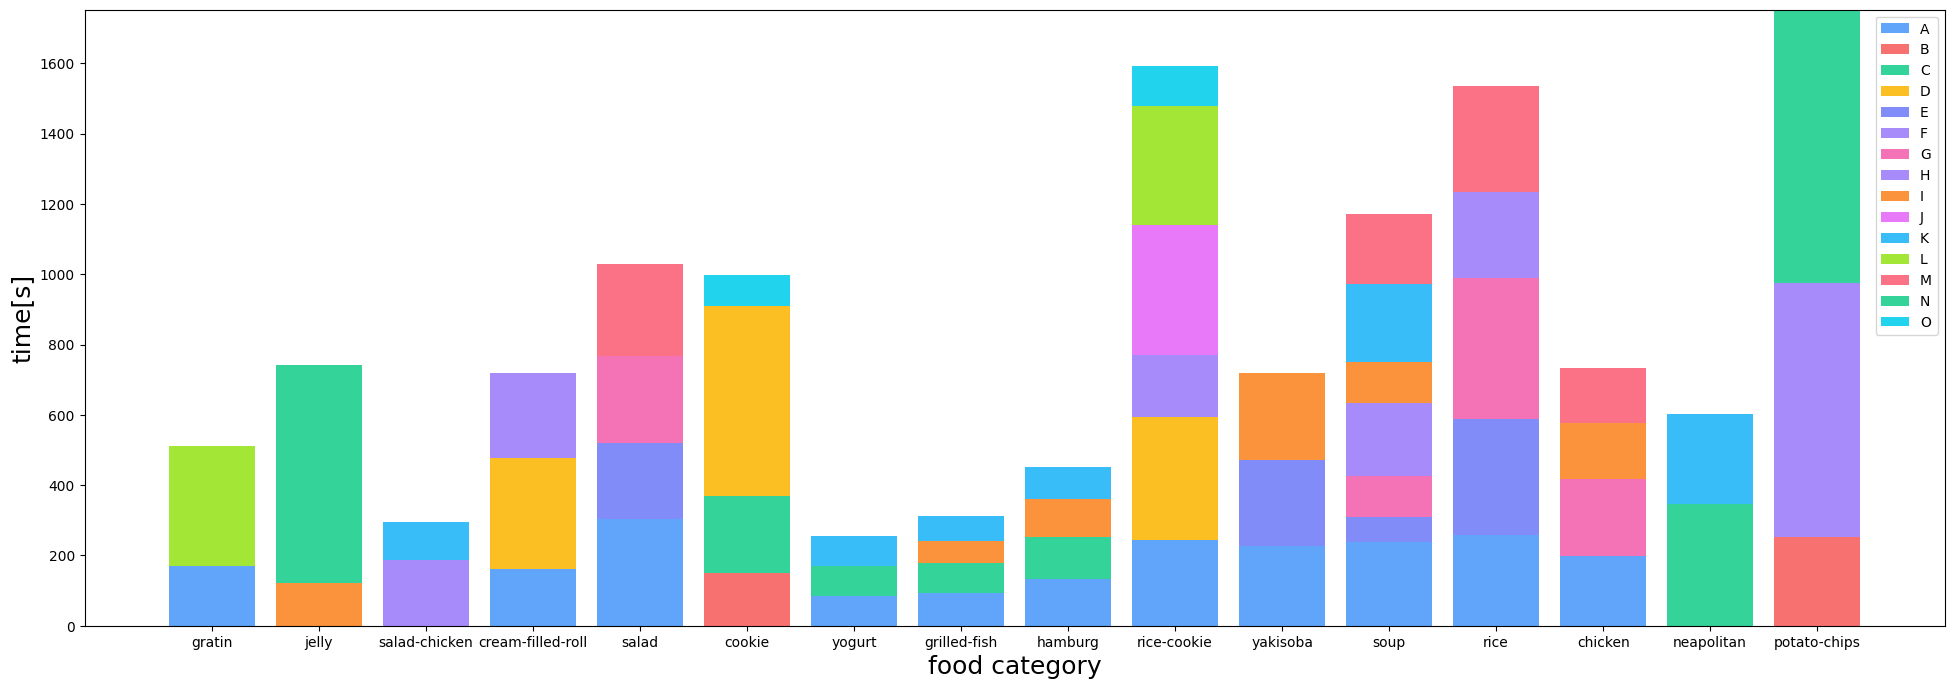
\includegraphics[clip,  width=0.9\hsize]{img/sound-data.png}
        \caption{食品毎の録音データ}
        \label{fig:sound-data}
    \end{center}
\end{figure*}

\begin{figure*}[t]
    \begin{minipage}[b]{0.16\hsize}
        \centering
        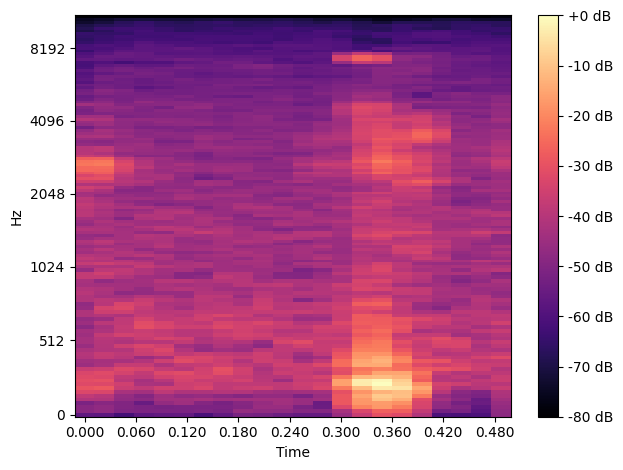
\includegraphics[width=\hsize]{img/melspec/chicken.png}
        \subcaption{唐揚げ}
    \end{minipage}
    \begin{minipage}[b]{0.16\hsize}
        \centering
        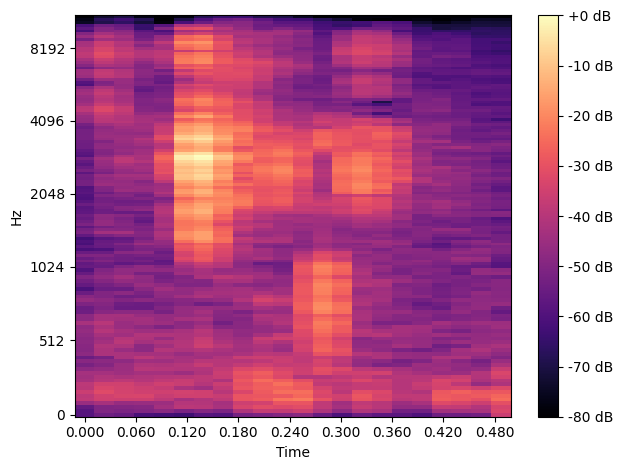
\includegraphics[width=\hsize]{img/melspec/rice.png}
        \subcaption{ご飯}
    \end{minipage}
    \begin{minipage}[b]{0.16\hsize}
        \centering
        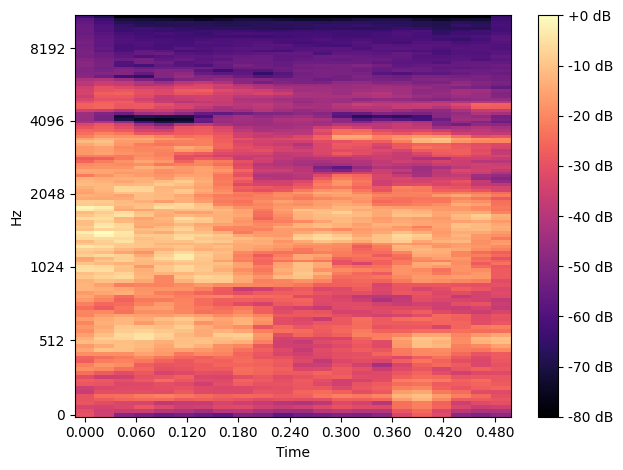
\includegraphics[width=\hsize]{img/melspec/soup.png}
        \subcaption{味噌汁}
    \end{minipage}
    \begin{minipage}[b]{0.16\hsize}
        \centering
        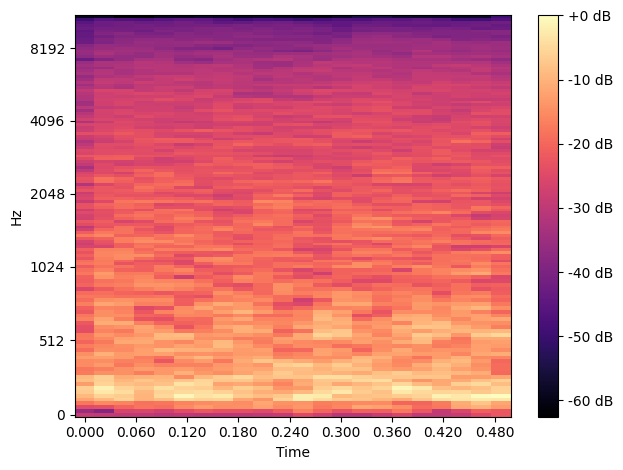
\includegraphics[width=\hsize]{img/melspec/salad.png}
        \subcaption{サラダ}
    \end{minipage}
    \begin{minipage}[b]{0.16\hsize}
        \centering
        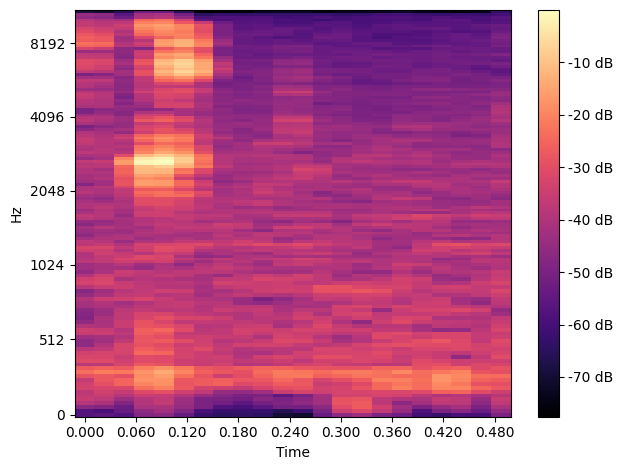
\includegraphics[width=\hsize]{img/melspec/rice-cookie.png}
        \subcaption{せんべい}
    \end{minipage}
    \begin{minipage}[b]{0.16\hsize}
        \centering
        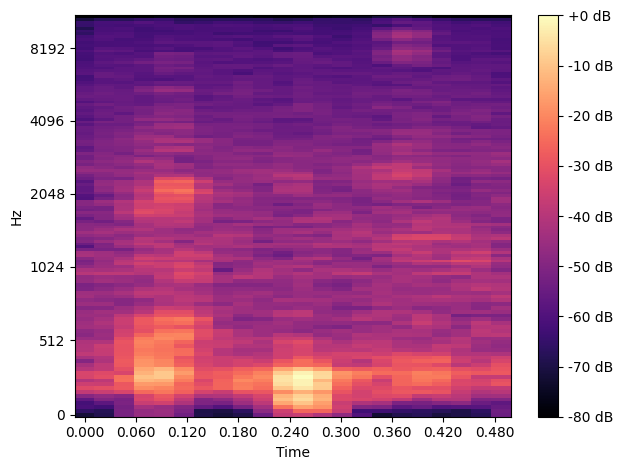
\includegraphics[width=\hsize]{img/melspec/gratin.png}
        \subcaption{グラタン}
    \end{minipage}
    \begin{minipage}[b]{0.16\hsize}
        \centering
        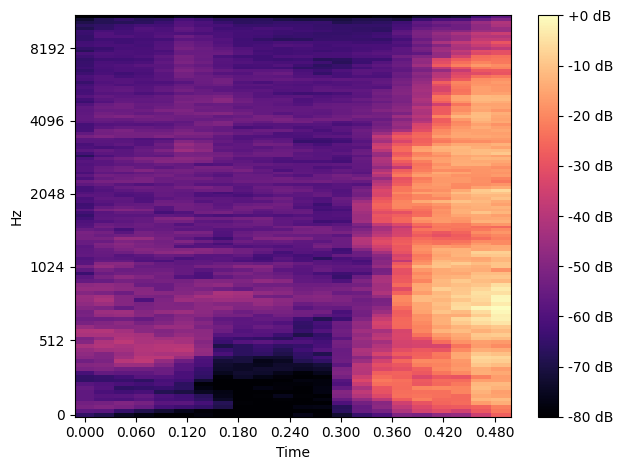
\includegraphics[width=\hsize]{img/melspec/cookie.png}
        \subcaption{クッキー}
    \end{minipage}
    \begin{minipage}[b]{0.16\hsize}
        \centering
        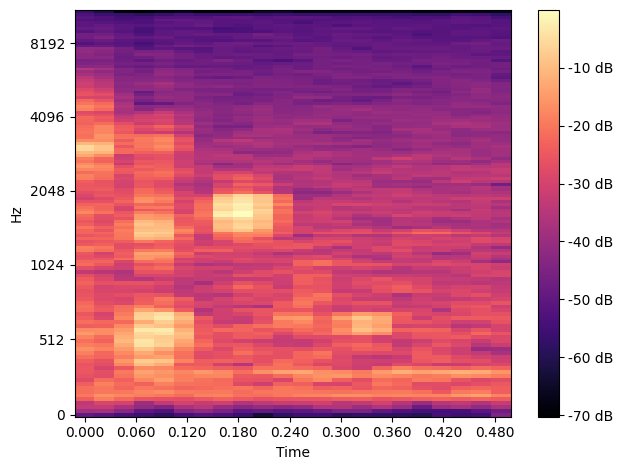
\includegraphics[width=\hsize]{img/melspec/potato-chips.png}
        \subcaption{ポテトチップス}
    \end{minipage}
    \begin{minipage}[b]{0.16\hsize}
        \centering
        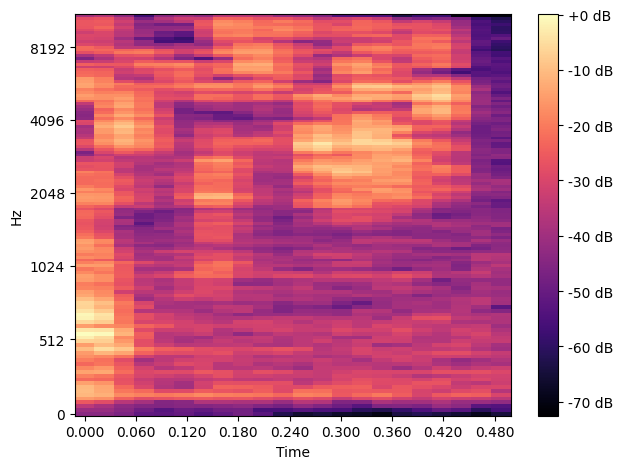
\includegraphics[width=\hsize]{img/melspec/neapolitan.png}
        \subcaption{スパゲティ}
    \end{minipage}
    \begin{minipage}[b]{0.16\hsize}
        \centering
        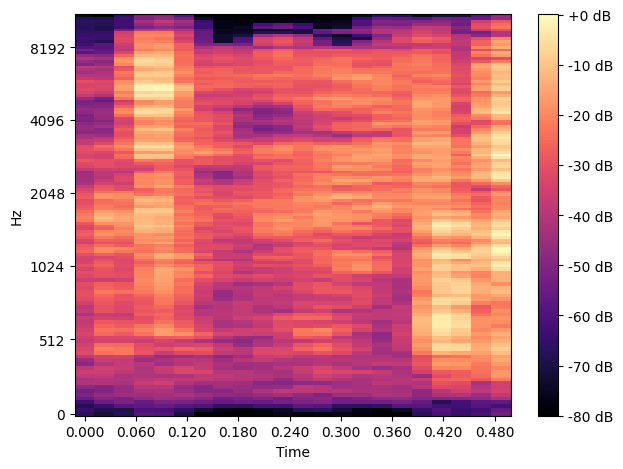
\includegraphics[width=\hsize]{img/melspec/yogurt.png}
        \subcaption{ヨーグルト}
    \end{minipage}
    \begin{minipage}[b]{0.16\hsize}
        \centering
        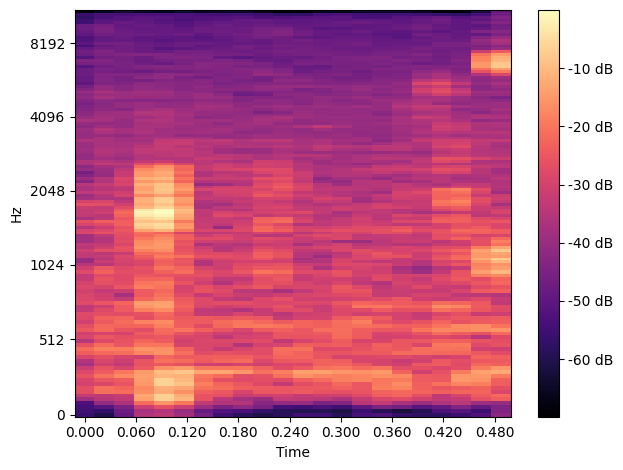
\includegraphics[width=\hsize]{img/melspec/hamburg.png}
        \subcaption{ハンバーグ}
    \end{minipage}
    \begin{minipage}[b]{0.16\hsize}
        \centering
        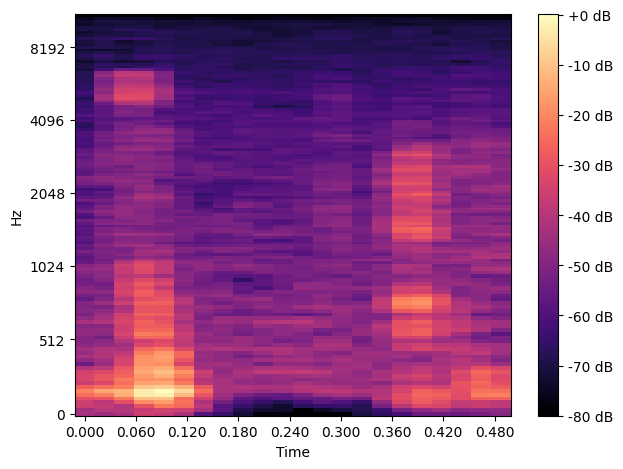
\includegraphics[width=\hsize]{img/melspec/salad-chicken.png}
        \subcaption{サラダチキン}
    \end{minipage}
    \begin{minipage}[b]{0.16\hsize}
        \centering
        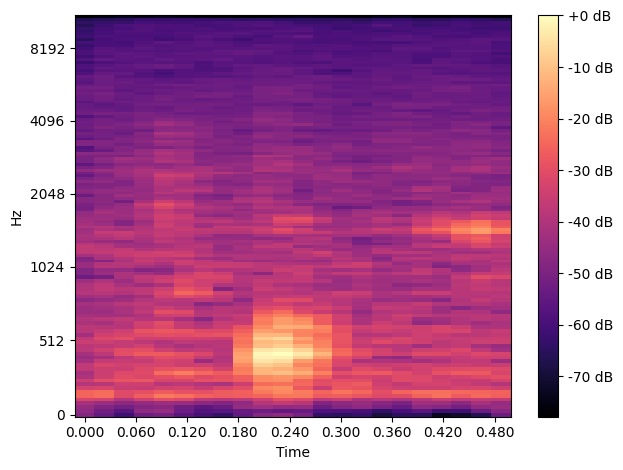
\includegraphics[width=\hsize]{img/melspec/cream-filled-roll.png}
        \subcaption{クリームパン}
    \end{minipage}
    \begin{minipage}[b]{0.16\hsize}
        \centering
        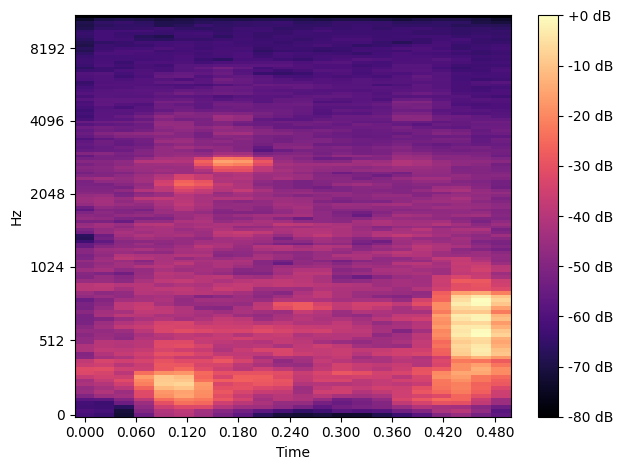
\includegraphics[width=\hsize]{img/melspec/yakisoba.png}
        \subcaption{焼きそば}
    \end{minipage}
    \begin{minipage}[b]{0.16\hsize}
        \centering
        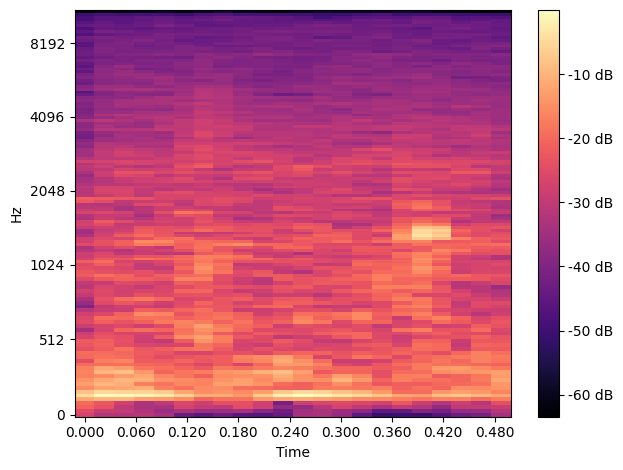
\includegraphics[width=\hsize]{img/melspec/jelly.png}
        \subcaption{ゼリー}
    \end{minipage}
    \begin{minipage}[b]{0.16\hsize}
        \centering
        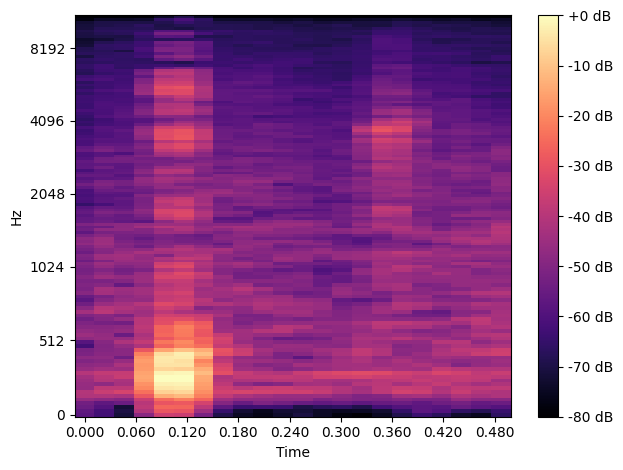
\includegraphics[width=\hsize]{img/melspec/grilled-fish.png}
        \subcaption{焼き魚}
    \end{minipage}
    \caption{録音データのメルスペクトログラムの一例}
    \label{fig:sample-melspec-data}
\end{figure*}

% 以下はRefTeX用
%%% Local Variables:
%%% mode: yatex
%%% TeX-master: "main"
%%% End:
